
\begin{center}
\Huge
Topunktsformlen for potensfunktioner og potensvækst
\end{center}
\section*{Topunktsformlen for potensfunktioner}
\stepcounter{section}
Som det var tilfældet med både lineære funktioner og eksponentialfunktioner, så er det også muligt at finde en entydig potensfunktion, der går gennem to givne punkter. Formlen for denne potensfunktion kalder vi for topunktsformlen for potensfunktioner.
\begin{setn}[Topunktsformlen for potensfunktioner]
Lad $(x_1,y_1)$ og $(x_2,y_2)$ være to punkter i første kvadrant. Så er der en entydig potensfunktion $f$, der skærer gennem disse punkter givet ved
\begin{align*}
f(x) = b\cdot x^a.
\end{align*}
Konstanterne $a$ og $b$ er givet ved henholdsvist
\begin{align*}
a = \frac{\log(y_2)-\log(y_1)}{\log(x_2)-\log(x_1)}
\end{align*}
og
\begin{align*}
b = \frac{y_1}{x_1^{a}}.
\end{align*}
\end{setn}
\begin{proof}
Fremgangsmåden er tilsvarende den, vi anvendte, da vi skulle udlede topunktsformlen for eksponentialfunktion. Vi antager derfor, at potensfunktionen $f$ givet ved
\begin{align*}
f(x) = b\cdot x^a
\end{align*}
går gennem punkterne $(x_1,y_1)$ og $(x_2,y_2)$. Vi må så have, at 
\begin{align*}
y_1 &= b\cdot x_1^a \textnormal{ og }\\ y_2 &= b\cdot x_2^a.
\end{align*}
Vi bestemmer nu forholdet mellen de to $y$-værdier:
\begin{align*}
\frac{y_2}{y_1} &= \frac{b\cdot x_2^a}{b\cdot x_1^a}\\
&= \frac{x_2^a}{x_1^a}\\
&= \left(\frac{x_2}{x_1}\right)^a.
\end{align*}
Vi kan nu isolere $a$ ved hjælp af totalslogaritmen $\log(x)$. (I princippet kunne vi også bruge $\ln(x)$ - det ville ingen forskel gøre.):
\begin{align*}
\frac{y_2}{y_1} = \left(\frac{x_2}{x_1}\right)^a &\Leftrightarrow \log\left(\frac{y_2}{y_1}\right) = \log\left(\left(\frac{x_2}{x_1}\right)^a\right) = a\log\left(\frac{x_2}{x_1}\right)\\
&\Leftrightarrow \frac{\log\left(\frac{y_2}{y_1}\right)}{\log\left(\frac{x_2}{x_1}\right)} = a\\
&\Leftrightarrow \frac{\log(y_2)-\log(y_1)}{\log(x_2)-\log(x_1)} = a,
\end{align*}
og vi har nu bestemt $a$. 
For at bestemme $b$ udnytter vi igen, at 
\begin{align*}
y_1 = b\cdot x_1^a \Leftrightarrow b = \frac{y_1}{x_1^a}.
\end{align*} 
\end{proof}
\begin{exa}
Lad os betragte et eksempel. Vi ønsker at finde den potensfunktion, der går gennem punkterne $(2,16)$ og  $(3,36)$. 
Vi bruger topunktsformlen til først at bestemme $a$.
\begin{align*}
a = \frac{\log(36)-\log(16)}{\log(3)-\log(2)} = 2.
\end{align*}
Dette bestemmes med CAS-værktøj som eksempelvist Maple. 
Vi bestemmer nu $b$:
\begin{align*}
b = \frac{16}{2^2} = \frac{16}{4} = 4.
\end{align*}
Potensfunktionen, der går gennem punkterne  $(2,16)$ og  $(3,36)$ er derfor bestemt ved
\begin{align*}
f(x) = 4\cdot x^2.
\end{align*}
På Fig. \ref{fig:topunktpotens} ses funktionen $f(x)$ samt de to regressionspunkter. 
\begin{figure}[H]
\centering
\begin{tikzpicture}
\begin{axis}[axis lines = middle,
 xmin = 0, ymin = 0]
\addplot[color = blue!40,samples = 1000] {4*x^2};
\node[circle, fill = red!40, inner sep = 0pt, minimum size=2mm] at (axis cs:2,16) {};
\node[circle, fill = red!40, inner sep = 0pt, minimum size=2mm] at (axis cs:3,36) {};
\legend{$f(x)=4\cdot x^2$}
\end{axis}
\end{tikzpicture}
\caption{Regression på de to punkter $(2,16)$ og $(3,36)$.}
\label{fig:topunktpotens}
\end{figure}
\end{exa}
\subsection*{Opgave 1}
\begin{enumerate}[label=\roman*)]

\item Brug topunktsformlen til at bestemme den potensfunktion, der går gennem punkterne $(0.5,1)$, og $(1.5,1.5)$.
\item Brug topunktsformlen til at bestemme den potensfunktion, der går gennem punkterne $(1,1)$ og $(2,2)$.

\item Grafen for en potensfunktion $f$ skærer gennem punkterne $(1,4)$ og $(2,9)$. Bestem forskriften for $f$
\item Grafen for en potensfunktion $g$ skærrer gennem punkterne $(3,10)$ og $(5,2)$. Bestem forskriften for $g$.
\item En potensfunktion $h$ opfylder, at $h(4)=15$ og $h(10) = 2$. Bestem forskriften for $h$.
\end{enumerate}

\subsection*{Opgave 2}
På Figur \ref{fig:potensopg} kan grafen for en potensfunktion $f$ ses. 
\begin{figure}[H]
	\centering
	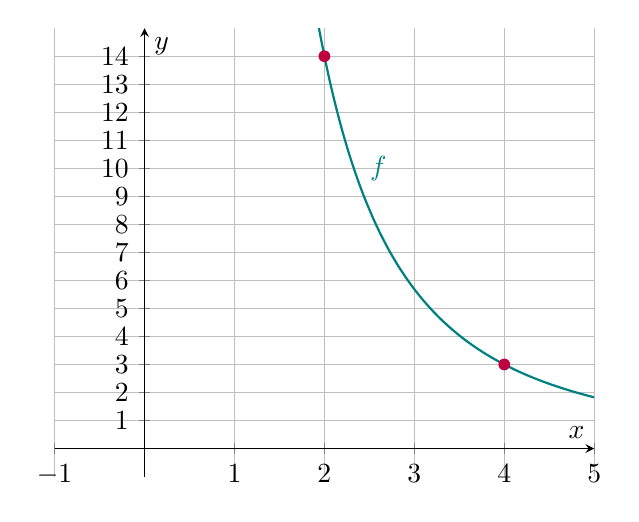
\begin{tikzpicture}
		\begin{axis}[
			axis lines = middle, 
			xmin = -1, xmax = 5,
			ymin = -1, ymax = 15,
			grid = both,
			ytick = {1,2,...,14},
			xlabel = {$x$},
			ylabel = {$y$}
			]
			\addplot[thick, color = teal, samples = 200, domain = 0.4:5]
			{65.333*x^(-2.2224)};
			\node[circle, fill, inner sep = 1.5pt, color = purple] at (axis cs:2,14){};
			\node[circle, fill, inner sep = 1.5pt, color = purple] at (axis cs:4,3){};
			\node[color = teal] at (axis cs:2.6,10) {$f$};
		\end{axis}
	\end{tikzpicture}
	\caption{Graf for potensfunktion $f$.}
	\label{fig:potensopg}
\end{figure}

\begin{enumerate}[label=\roman*)]
	\item Bestem en forskrift for $f$ ved at bruge topunnktsformlen for potensfunktioner
	\item Bestem $f(3)$ og undersøg, om dette passer med Figur \ref{fig:potensopg}.
	\item Løs ligningen $f(x) = 12$.
\end{enumerate}




\subsection*{Opgave 3}
\begin{enumerate}
	\item Potensfunktionen $f(x) = 2\cdot x^a$ går gennem punktet $(2,18)$. Brug dette til at bestemme $a$.
	\item Potensfunktionen $f(x) = b\cdot x^1$ går gennem punktet $(3,3)$. Brug dette til at bestemme $b$.
\end{enumerate}

\subsection*{Opgave 4}
Det antages, at bremselængden som funktion af hastigheden for en bil er en potenssammenhæng. For en bestemt bil er bremselængden ved 80km/t på 27.4 meter. Ved hastigheden 95km/t er bremselængden 38.7 meter.
\begin{enumerate}[label=\roman*)]
	\item Bestem en potensfunktion der beskriver bremselængden for bilen som funktion af tiden.
	\item Hvad vil bremselængden være for en bil, der kører 130km/t?
	\item Hvor stærkt skal man køre, hvis bremselængden skal være på 200m?
\end{enumerate}